\documentclass{standalone}
\usepackage{tikz}
\usepackage{schemabloc}

\begin{document}

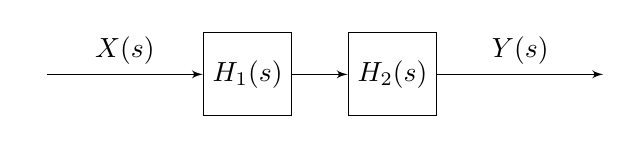
\begin{tikzpicture}
  % Entrée
  \sbEntree{E}
  % Premier bloc
  \sbBloc[6]{B1}{$H_1(s)$}{E}
  \sbRelier[$X(s)$]{E}{B1}
  % Deuxième bloc
  \sbBloc{B2}{$H_2(s)$}{B1}
  \sbRelier{B1}{B2}
  % Sortie
  \sbSortie[6]{S}{B2}
  \sbRelier[$Y(s)$]{B2}{S}
\end{tikzpicture}

\end{document}
